\section{MCU}\label{sec:mcu-hw}

		\subsection{The choosen MCU}\label{ssec:the-choosen-mcu}

		The system will be microcontrolled rather than microprocessed because this is the most practical way to ensure that the real-time constrain will be respected. The choosen microcontroller is the \textit{ATMEGA328PB} developed by \textit{Microchip} with 32 Kb of flash memory, 1 Kb of \textit{EEPROM} (Electrically Erasable Programmable Read-Only Memory), 2Kb of \textit{SRAM} (Static Random Access Memory), 27 GPIOs, 32 general purpose registers, five flexible timer/counters, two USARTs, 8-channel 10bit ADC \cite{atmega328p-datasheet}. 
		\par
		This microncontroller is widely used in academic environment (specially after the Arduino project started, when microncontroller programming became much more feasible and reachable), and is famous for being easy and reliable to use. The \textit{ATmega328p} has eight ADC inputs with a resolution of 10 bits and more 27 GPIO ports. This microcontroller also has a UART (explained in Section \ref{sssec:uart}). It is really versatile and more important it meets this project requirements, listed in Section \ref{sec:functionalRequirements}. This microcontroller will be used with a five volts supply, giving digital inputs and outputs a standard high logic level of five volts and low logic level of zero volts. The Figure \ref{fig:atmega328pb} shows the pinout of this device.

		\begin{figure}[htbp]
			\centering
			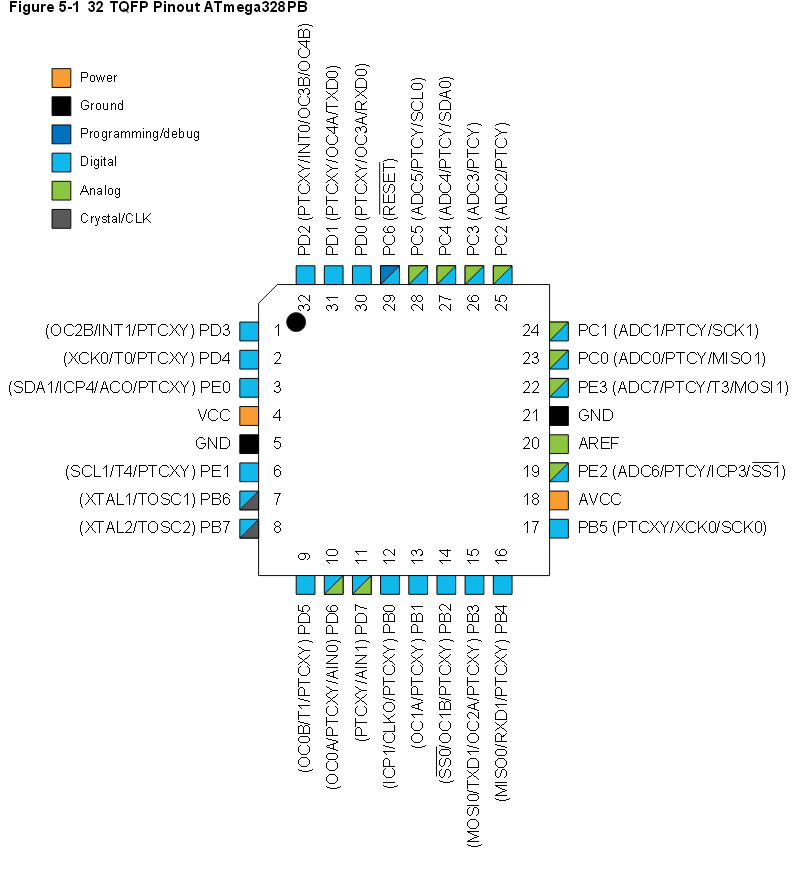
\includegraphics[scale=0.7]{figuras/fig-atmega328pb.png}
			\caption{\textit{ATmega238PB} pinout \cite{atmega328p-datasheet}}
			\label{fig:atmega328pb}
		\end{figure}
		

		\subsection{MCU circuit}\label{ssec:mcu-circuit}

		Figure \ref{fig:mcu-circuit} shows the complete complementary circuit for the MCU.

		\begin{figure}[htbp]
			\centering
			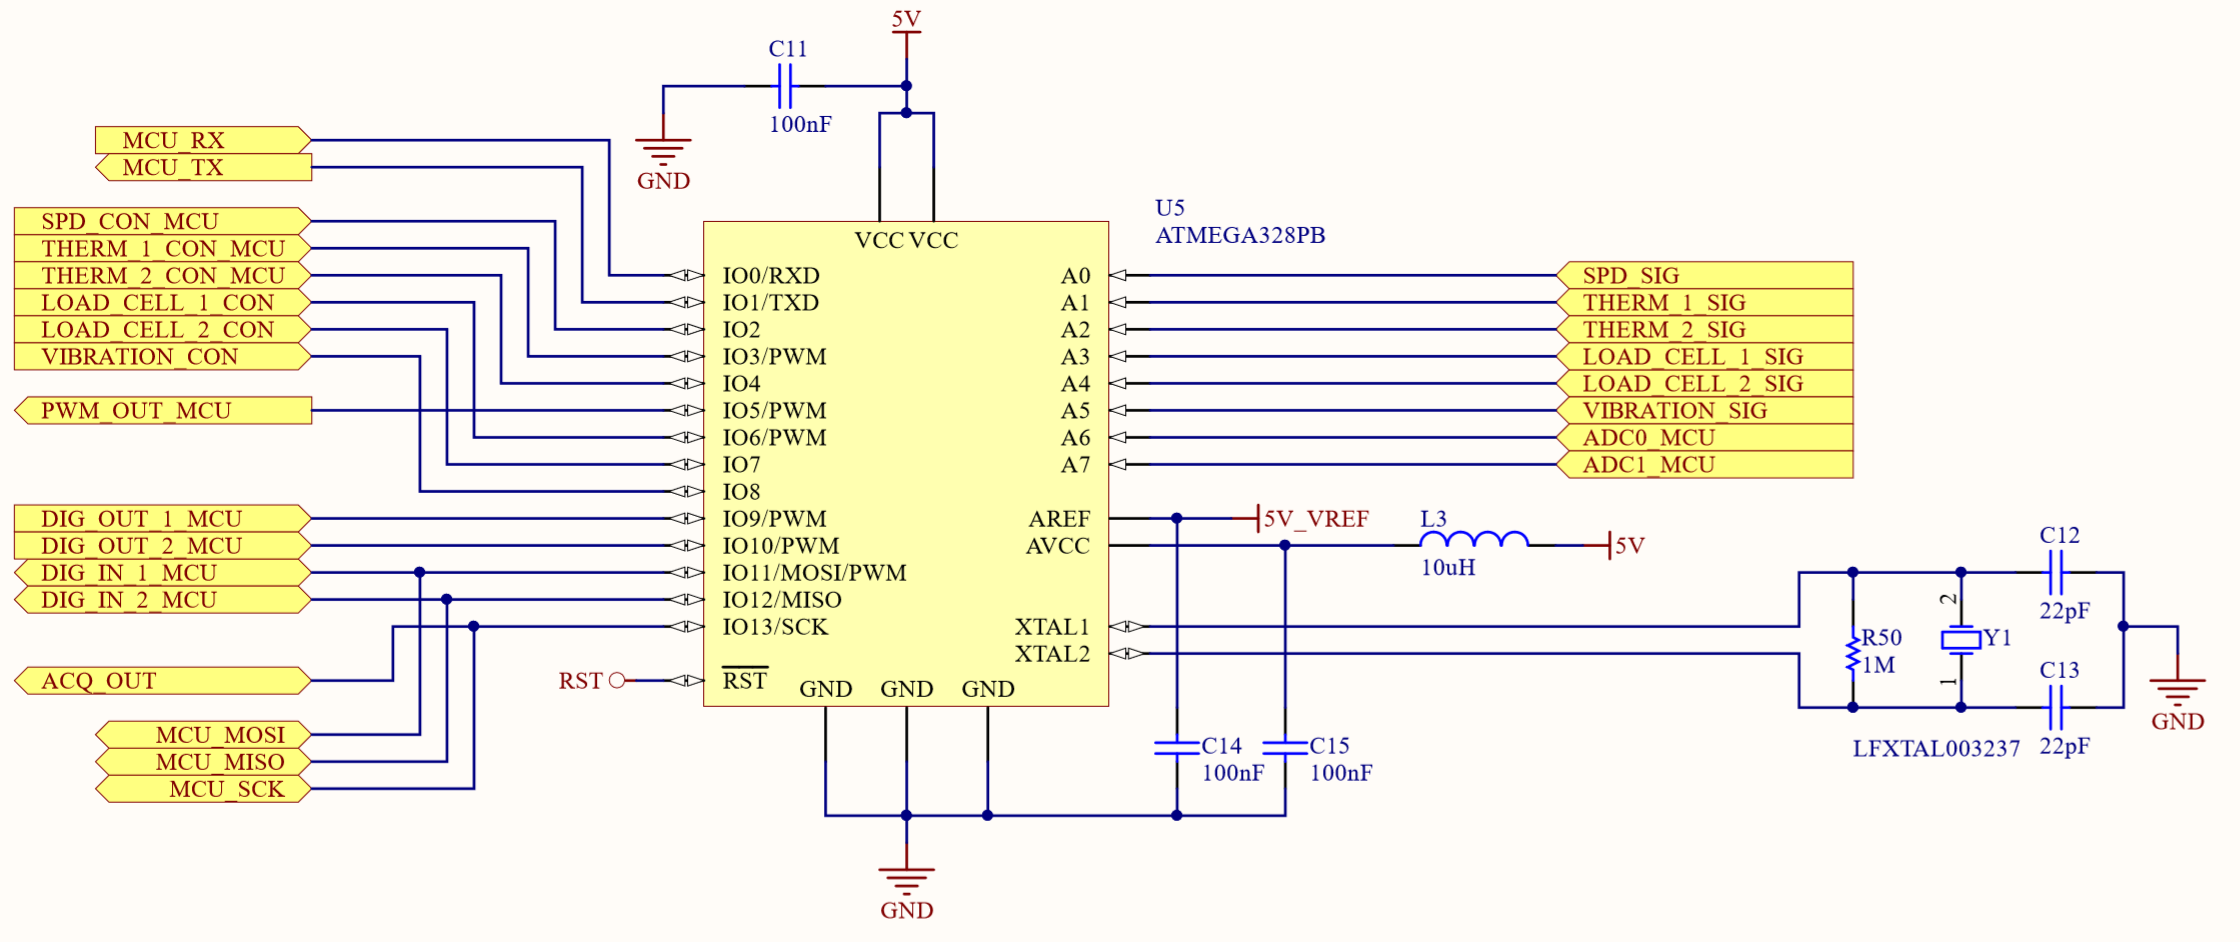
\includegraphics[scale=0.7]{figuras/fig-mcu-circuit.png}
			\caption{MCU Complete Complementary Circuit \cite{mcu-circuit}}
			\label{fig:mcu-circuit}
		\end{figure}

			\subsubsection{MCU Communication Ports}\label{sssec:mcu-com-ports}
				The ports in yellow and the RST ports are the MCU communication connections with other circuit modules, they are described as it follows.

				\begin{itemize}
					\item \textit{MCU_RX (input):} This port is used for receiving the serial data from the USB/UART circuit, as it was explained in Section \ref{ssec:usb-uart-complete-circuit}.\label{itm:mcu-port-mcu-rx}
					\item \textit{MCU_TX (output):} This port is used for transmitting the serial data to the USB/UART circuit, as it was explained in Section \ref{ssec:usb-uart-complete-circuit}.\label{itm:mcu-port-mcu-tx}
					\item \textit{SPD_CON_MCU (input):} A signal coming from the speed acquisition channel (Section \ref{ssec:ckp-sensor-detection-circuit}) that indicates whether the sensor in connected or not.\label{itm:mcu-port-spd-con-mcu}
					\item \textit{THERM_1_CON_MCU (input):} A signal coming from the first temperature acquisition channel (Section \ref{ssec:thermocouple-sensor-detection}) that indicates whether the sensor in connected or not.\label{itm:mcu-port-therm1-con-mcu}
					\item \textit{THERM_1_CON_MCU (input):} A signal coming from the second temperature acquisition channel (Section \ref{ssec:thermocouple-sensor-detection}) that indicates whether the sensor in connected or not.\label{itm:mcu-port-therm2-con-mcu}
					\item \textit{LOAD_CELL_1_MCU (input):} A signal coming from the first brake pressure acquisition channel (Section \ref{ssec:load-cell-sensor-detection}) that indicates whether the sensor in connected or not.\label{itm:mcu-port-load-cell-1-mcu}
					\item \textit{LOAD_CELL_2_MCU (input):} A signal coming from the second brake pressure acquisition channel (Section \ref{ssec:load-cell-sensor-detection}) that indicates whether the sensor in connected or not.\label{itm:mcu-port-load-cell-2-mcu}
					\item \textit{VIBRATION_CON (input):} A signal coming from the vibration acquisition channel (Section \ref{ssec:accelerometer-sensor-detection-circuit}) that indicates whether the sensor in connected or not.\label{itm:mcu-port-vibration-con}
					\item \textit{PWM_OUT_MCU (output):} This is a PWM signal that goes from the MCU to the DAC circuit in other to control the electric engine speed (Section \ref{ssec:pwm-to-speed-reference-circuit}).\label{itm:mcu-port-pwm-out-mcu}
					\item \textit{DIG_OUT_1_MCU (output):} First digital external output used in the circuit (Section \ref{ssec:digital-outputs}).\label{itm:mcu-port-dig-out-1-mcu}
					\item \textit{DIG_OUT_2_MCU (output):} Second digital external output used in the circuit (Section \ref{ssec:digital-outputs}).\label{itm:mcu-port-dig-out-2-mcu}
					\item \textit{DIG_IN_1_MCU (input):} First digital external input used in the circuit (Section \ref{ssec:digital-inputs}).\label{itm:mcu-port-dig-in-1-mcu}
					\item \textit{DIG_IN_2_MCU (input):} Second digital external input used in the circuit (Section \ref{ssec:digital-inputs}).\label{itm:mcu-port-dig-in-2-mcu} 
					\item \textit{ACQ_OUT (output):} Used to control a LED that blinks when signal acquisition is taking place (Section \ref{ssec:acquisition-led}).\label{itm:mcu-port-acq-out}   
					\item \textit{MCU_MOSI:} Used for ISP programming (Section \ref{sssec:microcontroller-isp-programming}).\label{itm:mcu-port-mcu-mosi}
					\item \textit{MCU_MISO:} Used for ISP programming (Section \ref{sssec:microcontroller-isp-programming}).\label{itm:mcu-port-mcu-miso}
					\item \textit{MCU_SCK:} Used for ISP programming (Section \ref{sssec:microcontroller-isp-programming}).\label{itm:mcu-port-mcu-sck}
					\item \textit{SPD_SIG: (input):} Analog input for the speed signal (Section \ref{ssec:ckp-signal-conditioning-circuit}).\label{itm:mcu-port-spd-sig}
					\item \textit{THERM_1_SIG: (input):} Analog input for the first temperature signal (Section \ref{ssec:thermocouple-signal-conditioning}).\label{itm:mcu-port-therm-1-sig}
					\item \textit{THERM_2_SIG (input):} Analog input for the second temperature signal (Section \ref{ssec:thermocouple-signal-conditioning}).\label{itm:mcu-port-therm-2-sig}
					\item \textit{LOAD_CELL_1_SIG (input):} Analog input for the first brake pressure signal (Section \ref{ssec:load-cell-signal-conditioning}).\label{itm:mcu-port-load-cell-1-sig}  
					\item \textit{LOAD_CELL_2_SIG (input):} Analog input for the second brake pressure signal (Section \ref{ssec:load-cell-signal-conditioning}).\label{itm:mcu-port-load-cell-2-sig} 
					\item \textit{VIBRATION_SIG (input):} Analog input for the vibration intensity signal (Section \ref{ssec:accelerometer-signal-conditioning-circuit}).\label{itm:mcu-port-vibration-sig}
					\item \textit{ADC0_MCU (input):} This port is not used and an internal MCU pull-up resistor is used.\label{itm:mcu-port-adc0-mcu}
					\item \textit{ADC1_MCU (input):} This port is not used and an internal MCU pull-up resistor is used.\label{itm:mcu-port-adc1-mcu}
					\item \textit{RST (input):} This is the reset connection for the MCU, used to reset the MCU using ISP programming.\label{itm:mcu-port-rst}
				\end{itemize}
		
			\subsubsection{MCU Power Ports}\label{sssec:mcu-power-ports}
				The MCU power ports are described as it follows, each power port funcion was taken from the components datasheet \cite{atmega328p-datasheet}. All voltage supplies have a 100nF decoupling capacitor also recommended by the MCU datasheet.

				\begin{itemize}
					\item \textit{VCC: } This is the main voltage supply port for the MCU, as mentioned in Section \ref {ssec:the-choosen-mcu} the MCU will be powered up with a 5V supply. More details of this supply line in Section \ref{sssec:5v-supply}.\label{itm:mcu-vcc}
					\item \textit{GND: } This is the ground reference for the MCU.\label{itm:mcu-gnd}
					\item \textit{AREF: } This is the analogic voltage reference for the ADC, a ADC is as good as it's voltage reference \cite{adc-good}. The net \textit{5V_VREF} is a precision 5V reference explained in Section \ref{sssec:5v-reference}.\label{itm:mcu-aref}
					\item \textit{AVCC: } This is the ADC power supply, the inductor was used to filter unwanted noise, and the usage of this inductor was based on the Arduino Uno Rev3 Schematic \cite{arduino-rev3-schematic}.\label{mcu-avcc}
				\end{itemize}

			\subsubsection{Crystal Oscilator Circuit}\label{sssec:mcu-crystal-oscilator}

				The MCU datasheet indicates the use of a external oscilation crystal, the additional components to the crystal were based on the Arduino Uno Rev3 \cite{arduino-rev3-schematic}.